\chapter{Chapter 2 Supplementary Content}\label{app:suppcontent}
\myappendices{Appendix \ref{app:suppcontent}: Chapter 2 Supplementary Content}
\newpage

\section{The Anatomical Fiducial Protocol}\label{app:AFIDs_supp}
The full AFIDs annotation protocol which can be access on: \url{https://afids.github.io/afids-protocol}. Figure \ref{fig:figuresupall_afids} provides a snippet of all 32 AFIDs in the three cardinal anatomical planes on the MNI2009bAsym template. 

\begin{figure}[hbt!]
    \centering
    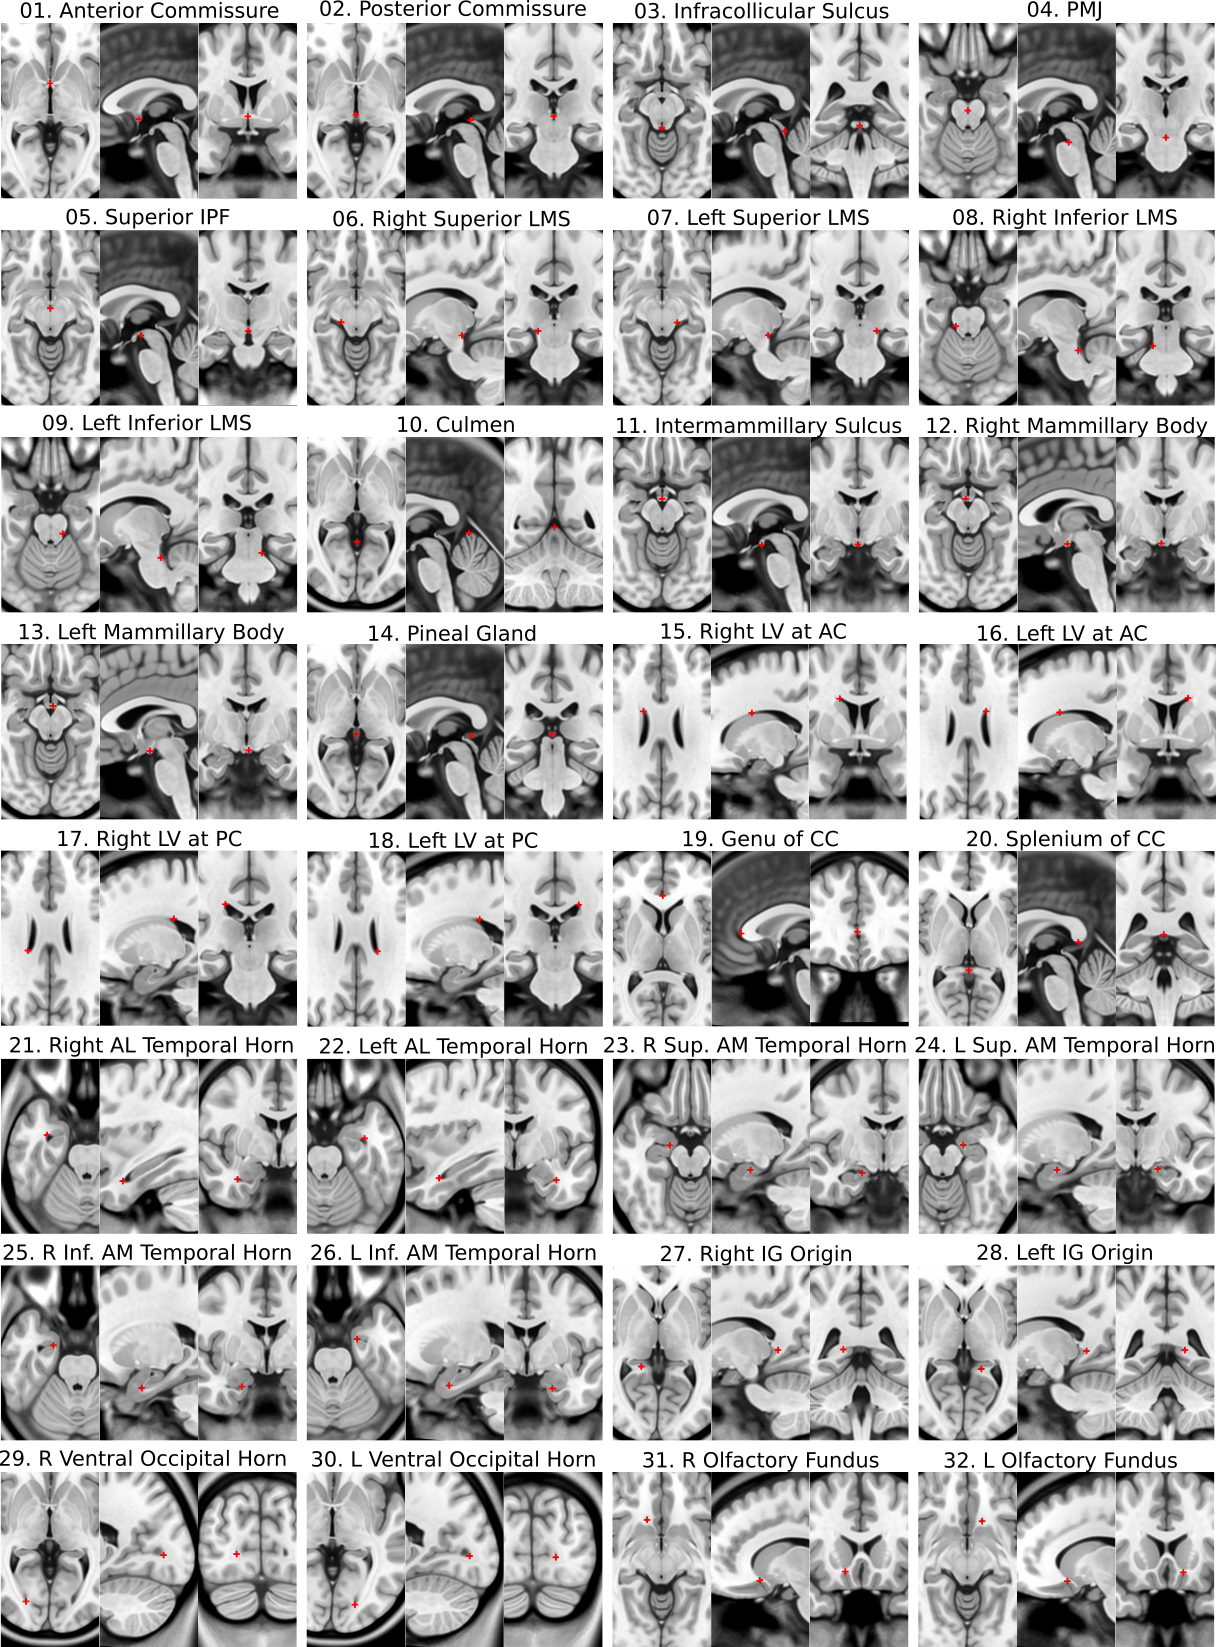
\includegraphics[width=0.8\linewidth]{figs/figuresupall_afids.png}
    \caption{The anatomical fiducials in the protocol is demonstrated with crosshairs at the representative location. AC, anterior commissure; AL, anterolateral; AM, anteromedial; IG, indusium griseum; IPF, interpeduncular fossa; LMS, lateral mesencephalic sulcus; LV, lateral ventricle; PC, posterior commissure; PMJ, pontomesenphalic junction.}
    \label{fig:figuresupall_afids}
\end{figure}


\newpage
\section{Rater Demographic Data}\label{app:rater_demo_data}
All annotations were performed by at least two human raters. As part of any annotation study, we collected demographic data on rater's experience in neuroanatomy, medical imaging, 3DSlicer software. Although not used in this paper, we also curated subthalamic nucelus (STN) segmentations on ultra-high field MRI (i.e., \(>\)7-T) data and add demographic rater data here for completeness. This data is used in Chapter \ref{chap:afidspred}. Table \ref{tab:rater_demographic_data} provides a breakdown of all the raters involved in datasets released in this work. 

\begin{table}[htbp]
\centering
\caption{
Summary of anatomical fiducial (AFID) and subthalamic nucleus (STN) annotation across datasets. Each row represents a unique annotator (Rater\_ID) contributing to one or more datasets. The table includes the experience (in months) of raters in three domains: Imaging, Neuroanatomy, and 3D Slicer. The diversity of rater backgrounds and annotation volumes reflects the breadth of participation across studies. Rater\_ID entries are context-specific and assigned uniquely within each dataset.
}
\begin{tabular}{llllll}
\toprule
Annotation & Dataset & Rater\_ID & Imaging & Neuroanatomy & 3DSlicer \\
\midrule
AFIDs & LHSCPD & AT & 0 & 0 & 0 \\
AFIDs & LHSCPD & GG & 60 & 60 & 60 \\
AFIDs & LHSCPD & MA & 60 & 60 & 60 \\
AFIDs & LHSCPD & MJ & 0 & 0 & 0 \\
AFIDs & LHSCPD & RC & 0 & 0 & 0 \\
AFIDs & AFIDs-HCP & AT & 60 & 60 & 60 \\
AFIDs & AFIDs-HCP & CZ & 12 & 12 & 12 \\
AFIDs & AFIDs-HCP & GG & 60 & 60 & 60 \\
AFIDs & AFIDs-HCP & DC & 24 & 24 & 24 \\
AFIDs & AFIDs-HCP & KF & 24 & 24 & 24 \\
AFIDs & SNSX32 & Rater01 & 12 & 12 & 12 \\
AFIDs & SNSX32 & Rater02 & 24 & 24 & 24 \\
AFIDs & SNSX32 & Rater03 & 24 & 24 & 24 \\
AFIDs & SNSX32 & Rater04 & 36 & 36 & 36 \\
AFIDs & SNSX32 & Rater05 & 24 & 24 & 24 \\
AFIDs & SNSX32 & Rater06 & 24 & 24 & 24 \\
AFIDs & SNSX32 & Rater07 & 24 & 24 & 24 \\
AFIDs & SNSX32 & Rater08 & 60 & 60 & 60 \\
AFIDs & SNSX32 & Rater09 & 12 & 12 & 12 \\
AFIDs & AFIDs-OASIS, MNI & Rater01 & 24 & 24 & 24 \\
AFIDs & AFIDs-OASIS, MNI & Rater02 & 0 & 0 & 0 \\
AFIDs & AFIDs-OASIS, MNI & Rater03 & 8 & 0 & 8 \\
AFIDs & AFIDs-OASIS, MNI & Rater04 & 24 & 6 & 0 \\
AFIDs & AFIDs-OASIS, MNI & Rater05 & 0 & 24 & 0 \\
AFIDs & AFIDs-OASIS, MNI & Rater06 & 24 & 12 & 12 \\
AFIDs & AFIDs-OASIS, MNI & Rater07 & 12 & 48 & 12 \\
AFIDs & AFIDs-OASIS, MNI & Rater08 & 0 & 0 & 0 \\
AFIDs & AFIDs-OASIS, MNI & Rater09 & 120 & 120 & 60 \\
AFIDs & 3T7T & Rater01 & 72 & 72 & 72 \\
AFIDs & 3T7T & Rater02 & 120 & 120 & 120 \\
AFIDs & 3T7T & Rater03 & 24 & 24 & 24 \\
AFIDs & 3T7T & Rater04 & 24 & 12 & 12 \\
AFIDs & 3T7T & Rater05 & 12 & 36 & 48 \\
AFIDs & 3T7T & Rater06 & 0 & 12 & 0 \\
STN & SNSX & Rater A & 120 & 120 & 60 \\
STN & SNSX & Rater B & 240 & 240 & 12 \\
STN & SNSX & Rater C & 72 & 72 & 72 \\
STN & 3T7T & Rater A & 84 & 84 & 84 \\
\bottomrule
\end{tabular}
\label{tab:rater_demographic_data}
\end{table}

\newpage

\section{The Anatomical Fiducial Protocol on T2w MRI}\label{app:AFIDs_T2w}

To date, no formal validation study has evaluated the application of the AFIDs protocol on T2w MRI. In this supplementary section, we demonstrate that localization of all 32 AFIDs is feasible on this imaging modality and that localization errors are comparable to prior validation studies \cite{Lau2019-eh,Abbass2022-lf}.

\subsection{Rater Characteristics and Annotation Procedure}

We recruited six human raters who completed the AFIDs protocol on T2w MRI scans from the 3T7T dataset described in Chapter \ref{chap:afidsdata}. An adapted protocol was curated for this purpose and is made available at: \url{https://ataha24.github.io/afids-protocol/afids_protocol/human_protocol_T2w.html}.

Three raters (rater1–rater3) were classified as experts, having prior experience with neuroanatomy, MRI, and the AFIDs protocol in previously published manuscripts. The remaining three (rater4–rater6) were novices with less than four years of experience and no prior exposure to AFID placement. All raters completed a demographic survey documenting their experience with neuroanatomy, MRI, and 3D Slicer which is provided here in Table~\ref{tab:rater_demographics_T2w} for completeness.

\begin{table}[ht]
\centering
\caption{Rater demographics including prior AFID placement experience and years of expertise in relevant domains for T2w AFID protocol validation.}
\begin{tabular}{lccccc}
\toprule
\textbf{Rater ID} & \textbf{Placed AFIDs Before?} & \textbf{Expert/Novice} & \textbf{3DSlicer} & \textbf{Neuroanatomy} & \textbf{MRI} \\
\midrule
1 & Y & Expert & 6 & 6 & 6 \\
2 & Y & Expert & 10 & 10 & 10 \\
3 & Y & Expert & 2 & 4 & 4 \\
4 & N & Novice & 2 & 1 & 1 \\
5 & N & Novice & 1 & 3 & 4 \\
6 & N & Novice & 0 & 1 & 0 \\
\bottomrule
\end{tabular}
\label{tab:rater_demographics_T2w}
\end{table}

\subsection{AFID Localization}

Raters placed the AFIDs protocol on 20 T2w MRI scans (10 at 3T and 10 at 7T) from 10 healthy participants. Localization accuracy was evaluated using the anatomical fiducial localization error (AFLE), defined as the Euclidean distance between a given rater’s placement and the mean coordinate across all raters for that fiducial. Across all scans and raters, the overall mean AFLE was $1.04 \pm 0.54$ mm. 

\subsection{AFLE Across Rater Group}
Expert raters localized AFIDs with a mean error of $1.01 \pm 0.72$ mm. Novice raters, following online training and protocol familiarization, achieved a mean error of $1.14 \pm 0.73$ mm. There were no statistically significant differences in AFLE between expert and novice raters via Wilcoxon signed-rank test.


\subsection{AFLE Across Scanner Group}
When stratified by scanner resolution, the median AFLE on 3T scans was 1.01 mm (IQR: 0.69 mm; mean: $1.08 \pm 0.51$ mm), while the median AFLE on 7T scans was 0.92 mm (IQR: 0.56 mm; mean: $0.99 \pm 0.56$ mm).
Wilcoxon signed-rank tests (significance threshold $p < 0.05$) revealed that AFLE was significantly lower on 7T scans for six fiducials:
\begin{itemize}[noitemsep]
    \item AFID 1 – anterior commissure
    \item AFID 2 – posterior commissure
    \item AFID 12 – right mamillary body
    \item AFID 13 – left mamillary body
    \item AFID 18 – left frontal horn
    \item AFID 31 – right occipital horn
\end{itemize}

Although 7T scans yielded significantly lower AFLE for a subset of AFIDs—likely reflecting enhanced anatomical contrast at ultra-high field strength—both 3T and 7T AFLE values fall well within the millimetric error range reported in prior validation studies. This suggests that while 7T imaging may offer marginal gains in anatomical resolution for specific landmarks, 3T scans remain sufficient to support reliable AFID localization. These findings reinforce the robustness of the AFIDs framework across field strengths and its generalizability to standard clinical MRI systems with T2w contrast.

\subsection{Conclusion}
This supplementary analysis confirms that AFID placement on T2w MRI is feasible and achieves millimetric accuracy across both clinical-grade (3T) and ultra-high field (7T) scans. Placement accuracy was comparable to previously published T1w-based studies \cite{Lau2019-eh,Abbass2022-lf} --- which ranged between 0-2 mm --- and novice raters were able to reach similar accuracy levels as expert annotators. These findings support the generalizability of the AFIDs protocol to T2w imaging for use in research and clinical neuroimaging workflows.


\newpage